\documentclass[UTF8]{EPURapport}
%\usepackage{listings}

%\renewcommand{\lstlistlistingname}{Liste des codes}
%\renewcommand{\lstlistingname}{Code}

%\addextratables{%
%	\lstlistoflistings
%}

%\swapAuthorsAndSupervisors

\thedocument{Cahier d'analyse}{Canne connectée pour aveugles}{}
\grade{Département Informatique\\ 5\ieme{} année\\ 2020-2021}
\authors{%
	\category{Auteurs}{%
		\name{Djawad M'DALLAH MARI} \mail{djawad.mdallah-mari@etu.univ-tours.fr}
	}
	\details{DII5 2020-2021}
}
\supervisors{%
	\category{Encadrants}{%
		\name{Gilles VENTURINI} \mail{gilles.venturini@etu.univ-tours.fr}
	}
	\details{Université François-Rabelais, Tours}
}
\abstracts{Cahier d'analyse canne connecée pour aveugles}
{}
{}
{}

\begin{document}

\chapter{Cahier d'analyse}

\section{Introduction}
Ce cahier d'analyse s'inscrit dans le cadre du projet Canne connectée pour aveugles. Il vise à présenter les analyses faites pour répondre aux besoins exprimés dans le cahier de spécifications. Une lecture au préalable du cahier de spécifications est donc recommandée afin de comprendre le contexte et les enjeux du projet.

Nous verrons donc dans ce document une analyse sur l'application Android à développer. Nous verrons en particulier quelques méthodes de reconnaissances d'objet pour le mobile, les différentes méthodes qui permettront d'informer l'utilisateur et également comment garantir à l'utilisateur une interface adaptée à ses contraintes.

\section{Reconnaissance d'objet}
\subsection{Librairies}
L'un des besoins primaires pour la réalisation de ce projet est la reconnaissance d'objet. Pour cela, il est important de choisir une librairie qui permet d'implémenter un réseau de neurones. Sur Android il existe l'Android Neural Networks API (NNAPI) qui est un API en C permettant de réaliser des opérations de machine learning. Il a été conçu pour fournir une couche de fonctionnalités bas niveau qui sera ensuite utilisable par des couches plus hauts niveau comme les frameworks TensorFlow ou encore Caffe2. Toutefois, il est tout à fait possible de faire abstraction des frameworks et implémenter une solution utilisant directement l'API. L'utilisation la plus commune est avec TensorFlow et plus précisément TensorFlow Lite qui est une version allégée de TensorFlow. Cette version allégée limite certaines opérations de TensorFlow lui permettant donc d'être utilisée pour les appareils embarqués. Il existe également Keras, un autre outil intéressant permettant de faire du machine learning. Cependant, dès lors que l'on souhaite déployer sur Android, il faudra passer par TensorFlow Lite et convertir le modèle en format TensorFlow Lite \footnote{\url{https://keras.io} : partie "Deploy Anywhere."}. Dans notre cas, l'utilisation de TensorFlow Lite pourrait suffir pour répondre à notre besoin. De plus, celle-ci dispose d'un large panel de modèles préentrainés comme on va le voir dans les parties qui suivent.  

\subsection{Modèles}
Un modèle est un fichier qui a été entrainé pour reconnaître certains types de motifs (pattern). Il est entrainé à partir d'un ensemble de données et utilise un algorithme qui lui permet "d'apprendre" à travers ces données. 

Le choix du bon modèle est un facteur important pour répondre au besoin de reconnaissance d'objet. En effet, toute l’application, pour qu'elle soit utile aux utilisateurs finals, dépend de la capacité du modèle à détecter et identifier un objet. Afin de répondre à ce besoin, il faudrait faire un inventaire des modèles de reconnaissance d'objet disponible puis faire des comparaisons. Pour mesurer les performances de chaque modèle, des critères doivent être établis (Latence, Disponibilité, Rapidité, Coût, ...) ainsi que des conditions de fonctionnement bien définis (caractéristique du smartphone, version d'android, version, ...). Cela permettrait d'avoir un environnement d'exécution commun pour chaque modèle et donc des mesures cohérentes.

\subsubsection{Modèles disponibles}
Avec la librairie TensorFlow, nous disposons d'un grand panel de modèles préentrainés. La plupart de ces modèles ne sont pas directement compatible avec TensorFlow Lite. Ceux sur TF2 Detection zoo \footnote{\url{https://github.com/tensorflow/models/blob/master/research/object_detection/g3doc/tf2_detection_zoo.md}} peuvent être converti en utilisant TFLite Converter \footnote{\url{https://www.tensorflow.org/lite/convert}}. Les modèles déjà adaptés TensorFlow Lite sont disponible sur le hub officiel de TensorFlow \footnote{\url{https://tfhub.dev}} mais peu de modèles de reconnaissance d'image y sont rescencés notamment de reconnaissance d'objets (\textbf{Object Detection}) \footnote{\url{https://tfhub.dev/s?deployment-format=lite&module-type=image-object-detection}}. En effet, il existe que trois modèles officiels dans cette catégorie : SSD MobileNet, Mobile Object Localizer et East Text Detector. Parmi ces trois modèles, on peut déjà abandonner le East Text Detector puisqu'il s'agit ici de détecter du texte. En revanche, d'autres modèles de reconnaissance d'objet sont disponibles sur le github de TensorFlow \footnote{\url{https://github.com/tensorflow/models/blob/master/research/object_detection/g3doc/tf1_detection_zoo.md}} et sont à priori déjà compatible mobile. Ces modèles là sont intéressants car ils n'ont pas tous été entraînés avec la même banque d'images, on pourra donc choisir celui qui répond le plus à notre besoin (voir partie \ref{choixmodele}). Au niveau des modèles de \textbf{Classification}, il existe un peu plus de modèles compatibles TensorFlow Lite \footnote{\url{https://tfhub.dev/s?deployment-format=lite&module-type=image-classification}}. Les modèles de classification, malgré le faite qu'ils sont plus précis, vont moins répondre à notre besoin initial, mais méritent d'être évoqués puisque ceux-ci pourraît être mis en place dans une version futur du projet en complément du modèle de reconnaissance d'objet choisi.

\subsubsection{Object Detection vs Classification}
Les modèles de reconnaissances d'objet (Objet Detection) sont capables de localiser et identifier plusieurs objets sur une même image.

\begin{figure}[h!]
\centering
  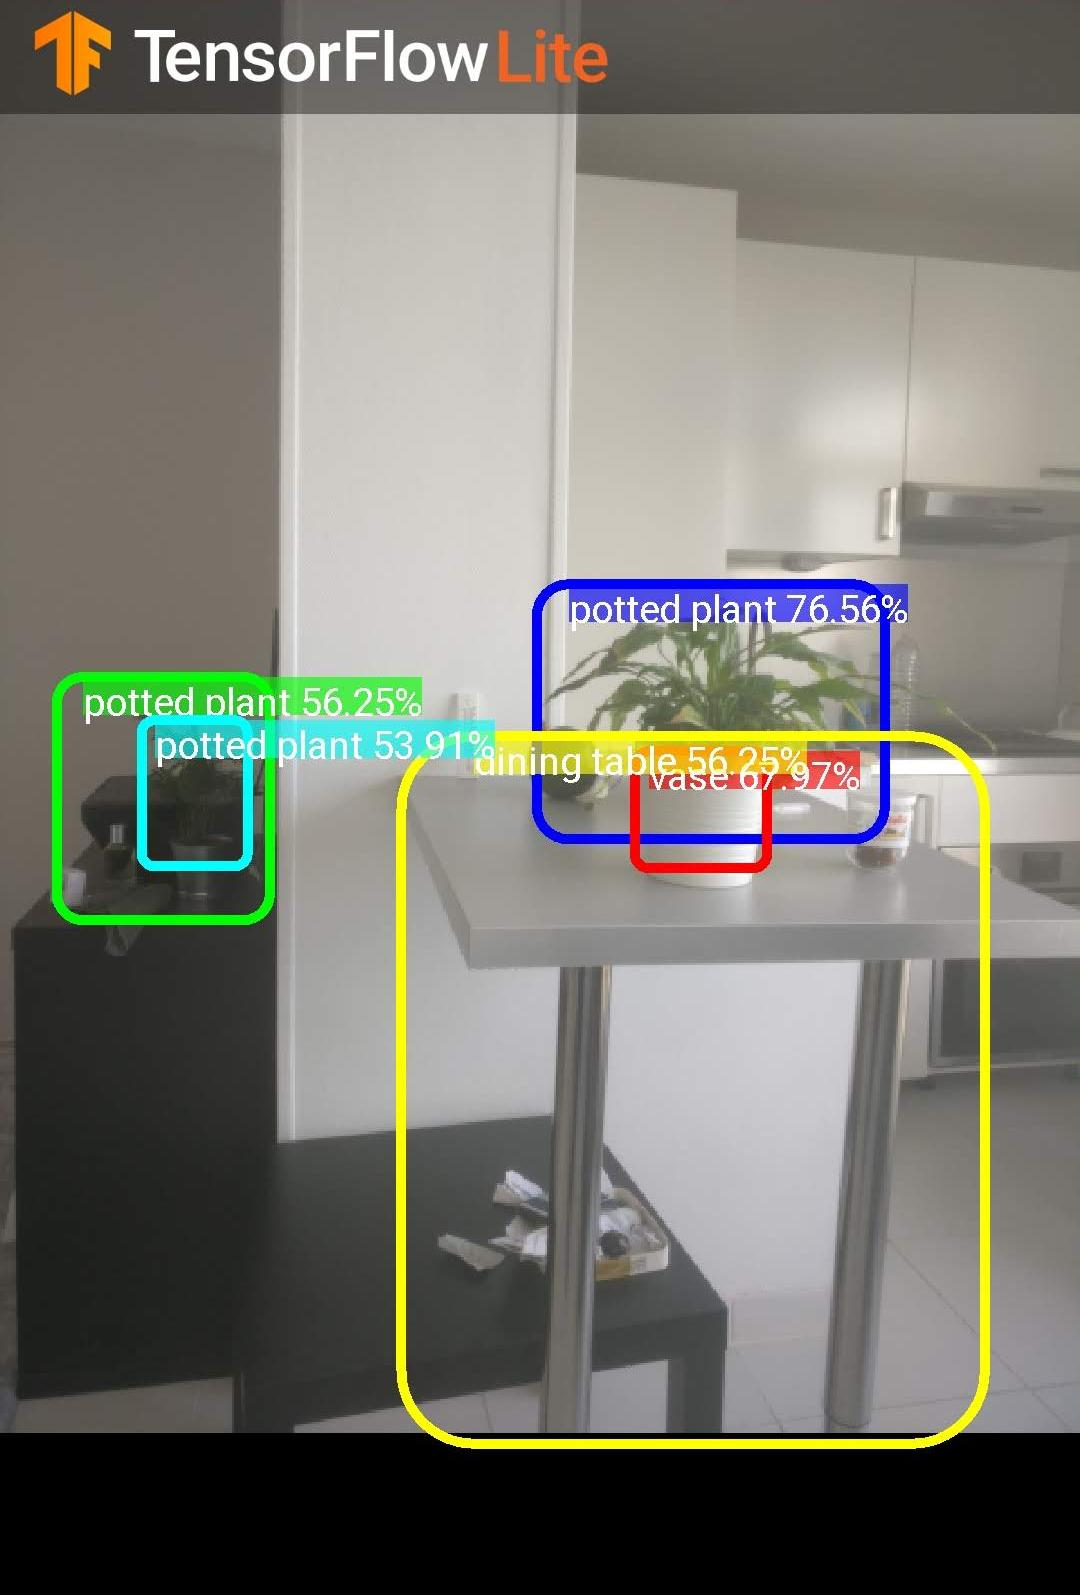
\includegraphics[width=0.7\textwidth]{images/object_detection.jpg}
  \caption{Exemple de reconnaissance d'objet}
  \label{fig:objectdetection}
\end{figure}

 Ce type de modèle est entraîné avec des objets de différentes classes (vêtements, fruits, etc.). Avec TensorFlow lorsqu'on met à l'éntrée de ce type de modèle une image, on obtient en sortie une liste d'objets avec chacun sa localisation, sa classe et un degré de confidence (qui correspond à la fiabilité de l'objet identifié).

\newpage
\begin{figure}[h!]
\centering
  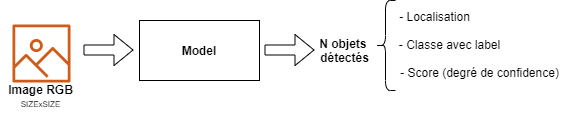
\includegraphics[width=0.6\textwidth]{images/schema_objectDetection.png}
  \caption{Schema principe de fonctionnement d'un modèle}
  \label{fig:schema_objectdetection}
\end{figure}

En revanche, les modèles de \textbf{classification} avec TensorFlow ne détecte qu'un seul élément sur une image. Ces modèles sont entraînés sur une seule classe générique (exemple : vêtements, aliments, plantes, etc) qui va ensuite être capable d'identifier l'élément de manière plus précise. Exemple : \\

\begin{itemize}
  \item Classe vêtements : T-shirt, jean, ...
  \item Classe aliments : salade, pâtes, ...
  \item Classe fruits : pomme, banane, ...  
  \item Classe insectes : sauterelle, abeille, papillon, ...
  \item  ...
\end{itemize}

\begin{figure}[h!]
\centering
  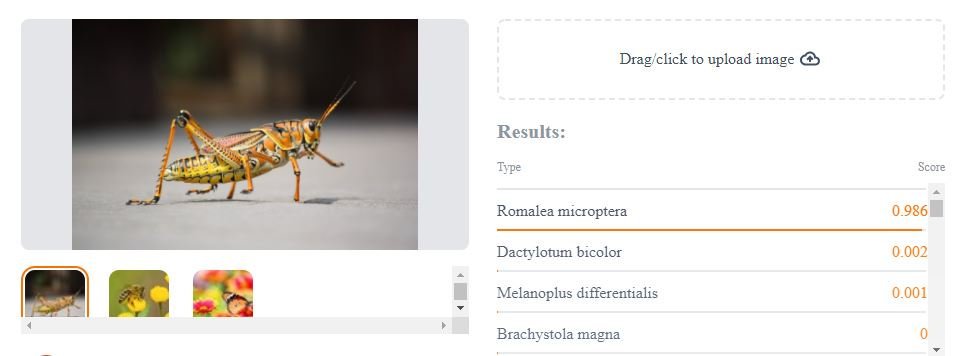
\includegraphics[width=\textwidth]{images/insects_classification.jpg}
  \caption{Exemple de classification d'insectes}
  \label{fig:insectsclassification}
\end{figure}

\subsubsection{Choix du modèle} \label{choixmodele}
Notre objectif pour notre premier prototype est d'utiliser un modèle qui reconnait un maximum d'objet dans différentes classes. Cela permettrait donc aux utilisateurs finaux de faire détecter un ensemble d'objet de différentes catégories plutôt que d'un catégorie spécifique. De ce point de vue, les modèles de classification tels qu'on les as vu précédemment ne correspondraient donc pas à ce besoin. Néanmoins, pour des versions ultérieurs de l'application, il pourra être envisager, soit une amélioration du modèle utilisé pour que celui-ci soit plus précis, ou ajouter la possibilité de changer de modèle. Il nous faut donc choisir parmi les deux modèles disponibles évoqués précedemment à savoir SSD MobileNet et Mobile Object Localizer.

Mobile Object Localizer

SSD MobileNet
Different mobileNet qui existe (changement minim): %https://github.com/tensorflow/models/blob/master/research/object_detection/g3doc/tf1_detection_zoo.md#mobile-models



notre besoin (max d'objet,existant,reliable..)
benchmark..
banque d'image
classification
Dans notre cas 
ident 1 objet à la X(objet id)
\subsection{Intégration dans une application Android}
les méthodes d'integration
fonctionnement
entrée sortie

\section{Informer l'utilisateur}
\subsection{Synthèse vocale}
fonctionnement
parametrage
rendre le message compréhensible: viseur,
vibreur
encodage-trame (1mots,phrase,1vib,2vib,vib long..?)
diag de classe

\subsection{Vibration}

\section{Navigation}
\subsection{Guide d'utilisation}
\subsection{Accès aux réglages}

\annexes

\end{document}